\subsection{Introduction}
This chapter presents a formal analysis of the application. Since the application domain is time dependent at its core, we decided to model the evolution of the system over time, with focus on the entrances to the Shops. The model focuses on Customers, Tickets and Bookings: the Staff can be seen as an intermediary and moderator between the Customers and the system, therefore, by assuming that the Staff will follow the rules, we can simplify the model for clarity and ease of comprehension.
The scenario being analyzed starts from a state in which Customers already have acquired the tokens and enter the Shops. The queue uses strict constraints, by allowing only the first in queue to enter the Shop. In practice, the constraint can be relaxed to increase throughput if needed. 
In particular, the model checks the following properties:
\begin{itemize}
    \item No department in a Shop exceeds its occupancy limits
    \item Customers cannot enter a Shop without a valid Token
    \item Customers can use a Booking to enter a Shop only at the time specified
    \item Customers cannot cut the waiting line for a Shop
    \item The same Token cannot be used for multiple visits
\end{itemize}
\subsection{Alloy code}
\subsubsection{Model description}
The first section describes the signatures of the objects which are relevant for the formal analysis and their representation invariants.
\lstinputlisting[language=alloy,firstline=1,lastline=68]{alloy/main.als}
\subsubsection{Dynamic properties}
This section describes the rules that guarantee the correct evolution of the system over time. In particular, the \texttt{Trace} fact rules the transition from an instant to the next for Customers and for the Waiting List. 
\lstinputlisting[language=alloy,firstline=72,lastline=127]{alloy/main.als}
\subsubsection{Assertions}
This section lists some of the property that will be guaranteed \emph{if} the invariants described in the previous sections hold. The The result of the evaluation of these assertions will be presented in the next section.
\lstinputlisting[language=alloy,firstline=131,lastline=211]{alloy/main.als}
\subsubsection{Execution results}
This section shows the experimental result of the formal analysis 
\lstinputlisting[language=alloy,firstline=215]{alloy/main.als}

\pagebreak
The following figures show the evolution of a particular instance of the enterAndExit predicate, for 5 consecutive Time instants. A visiting Customer is pointed out by a \emph{visiting} connection to one of the Visit elements, which, in turn, is connected to a set of Department nodes of the same Shop.
\begin{figure}[H]
    \centering
    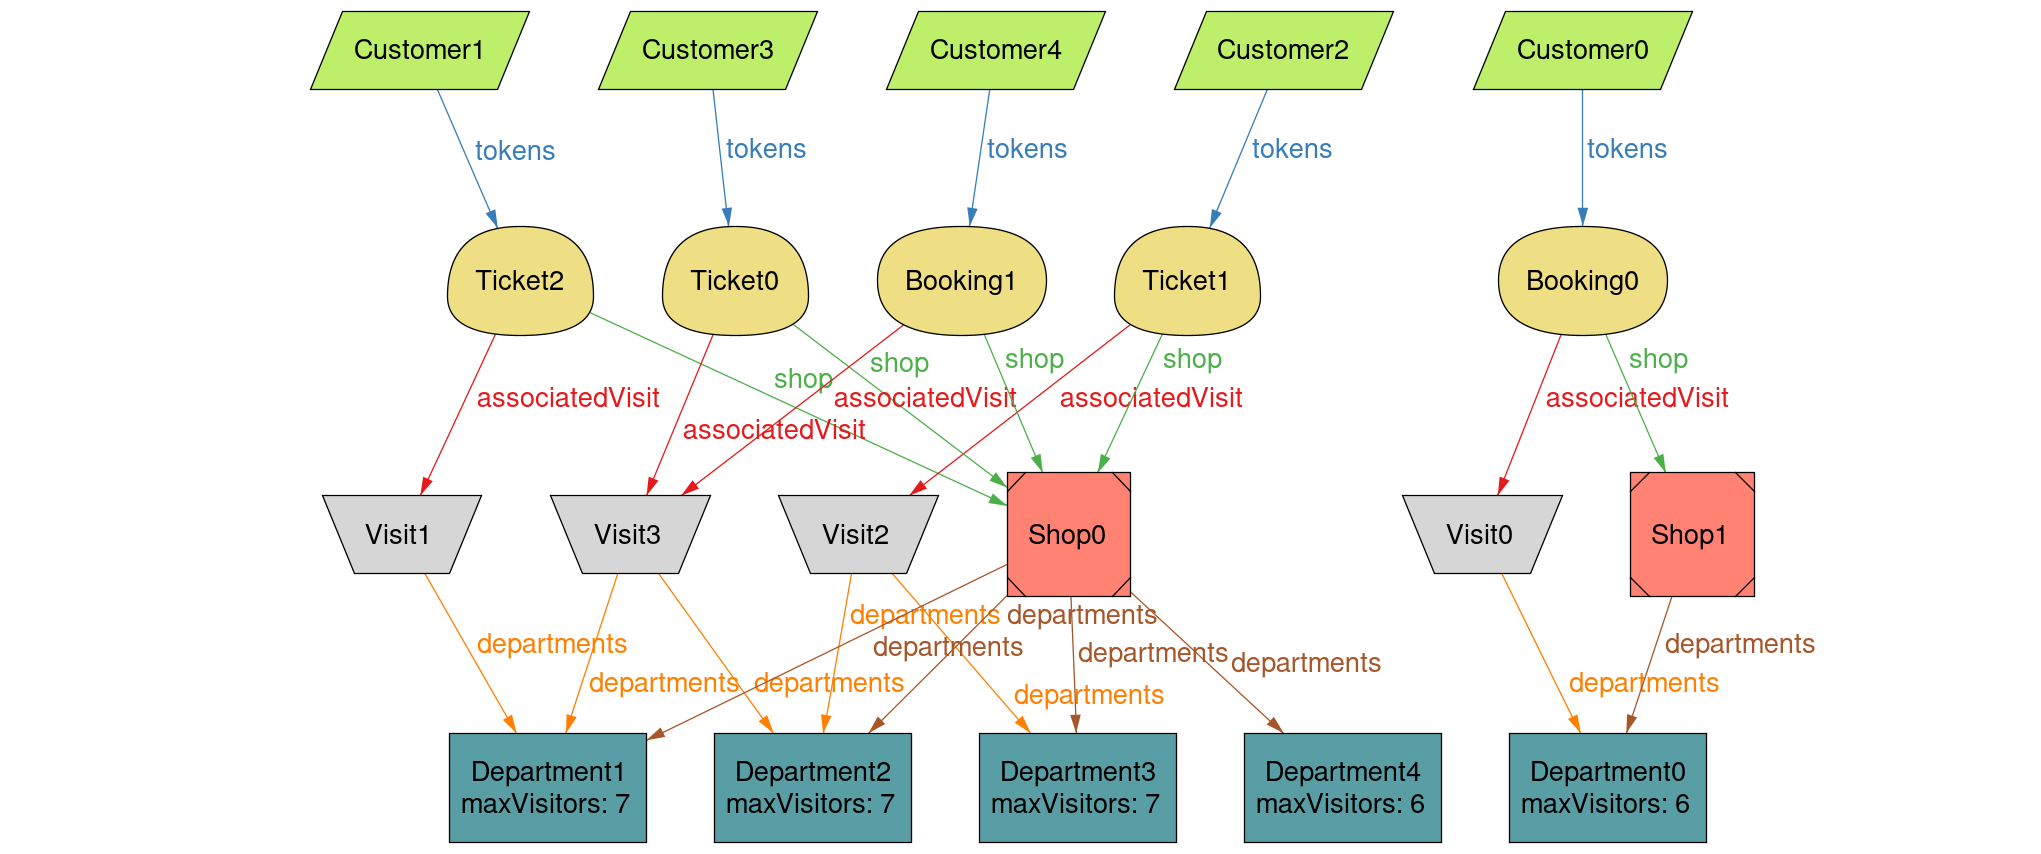
\includegraphics[height=0.25\textheight]{Images/Alloy/5Customers_v1_t0.png}
    \caption{Run for Time 0. This is the initial state.}
\end{figure}
\begin{figure}[H]
    \centering
    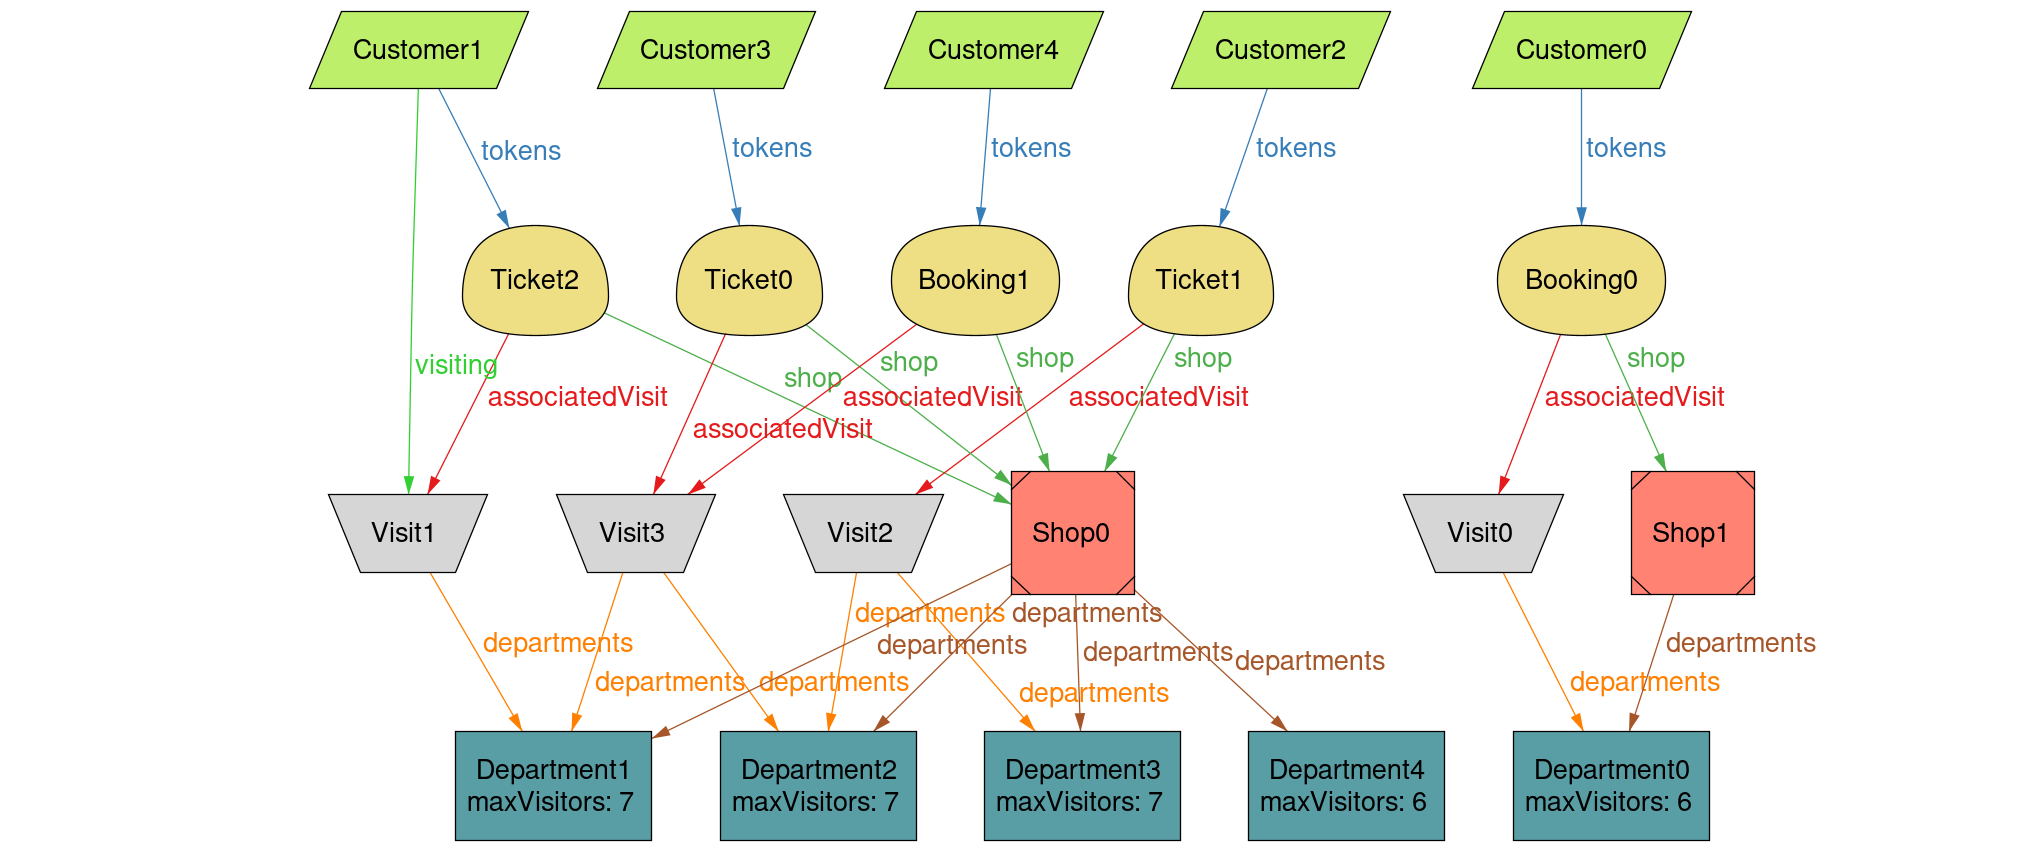
\includegraphics[height=0.25\textheight]{Images/Alloy/5Customers_v1_t1.png}
    \caption{Run for Time 1. \emph{Customer1} has used his Ticket to enter \emph{Shop0}.}
\end{figure}
\begin{figure}[H]
    \centering
    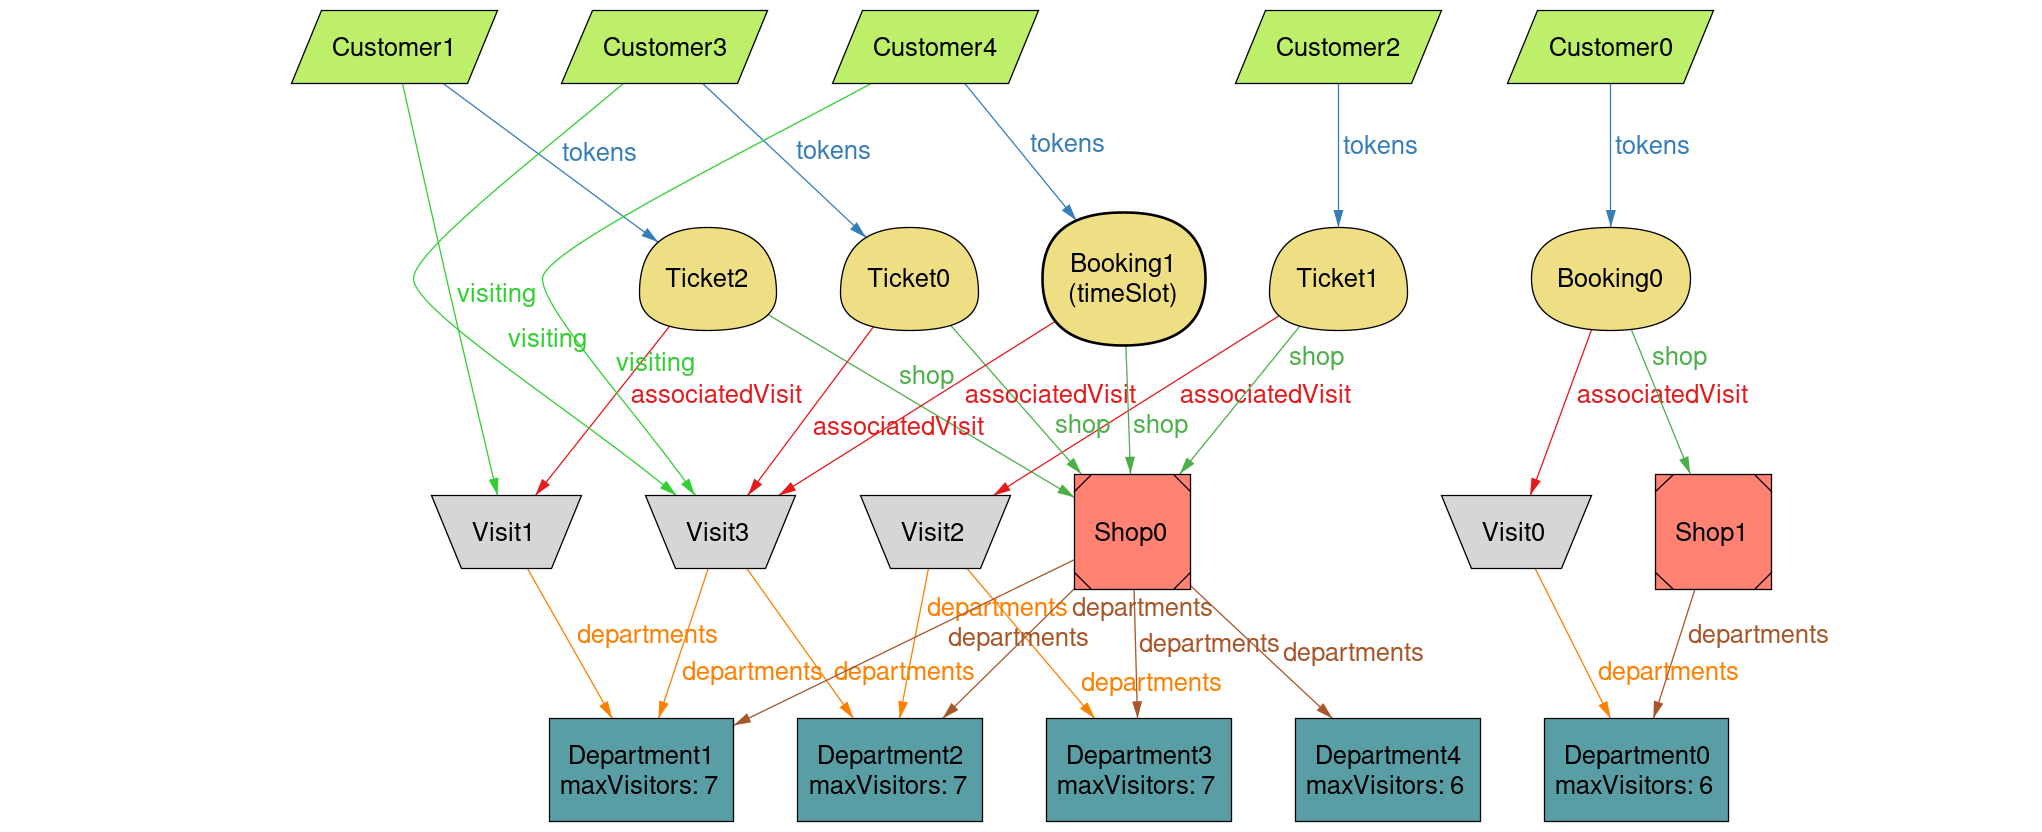
\includegraphics[height=0.25\textheight]{Images/Alloy/5Customers_v1_t2.png}
    \caption{Run for Time 2. \emph{Customer3} and \emph{4} enter the same shop with a Ticket and a Booking respectively.}
\end{figure}
\begin{figure}[H]
    \centering
    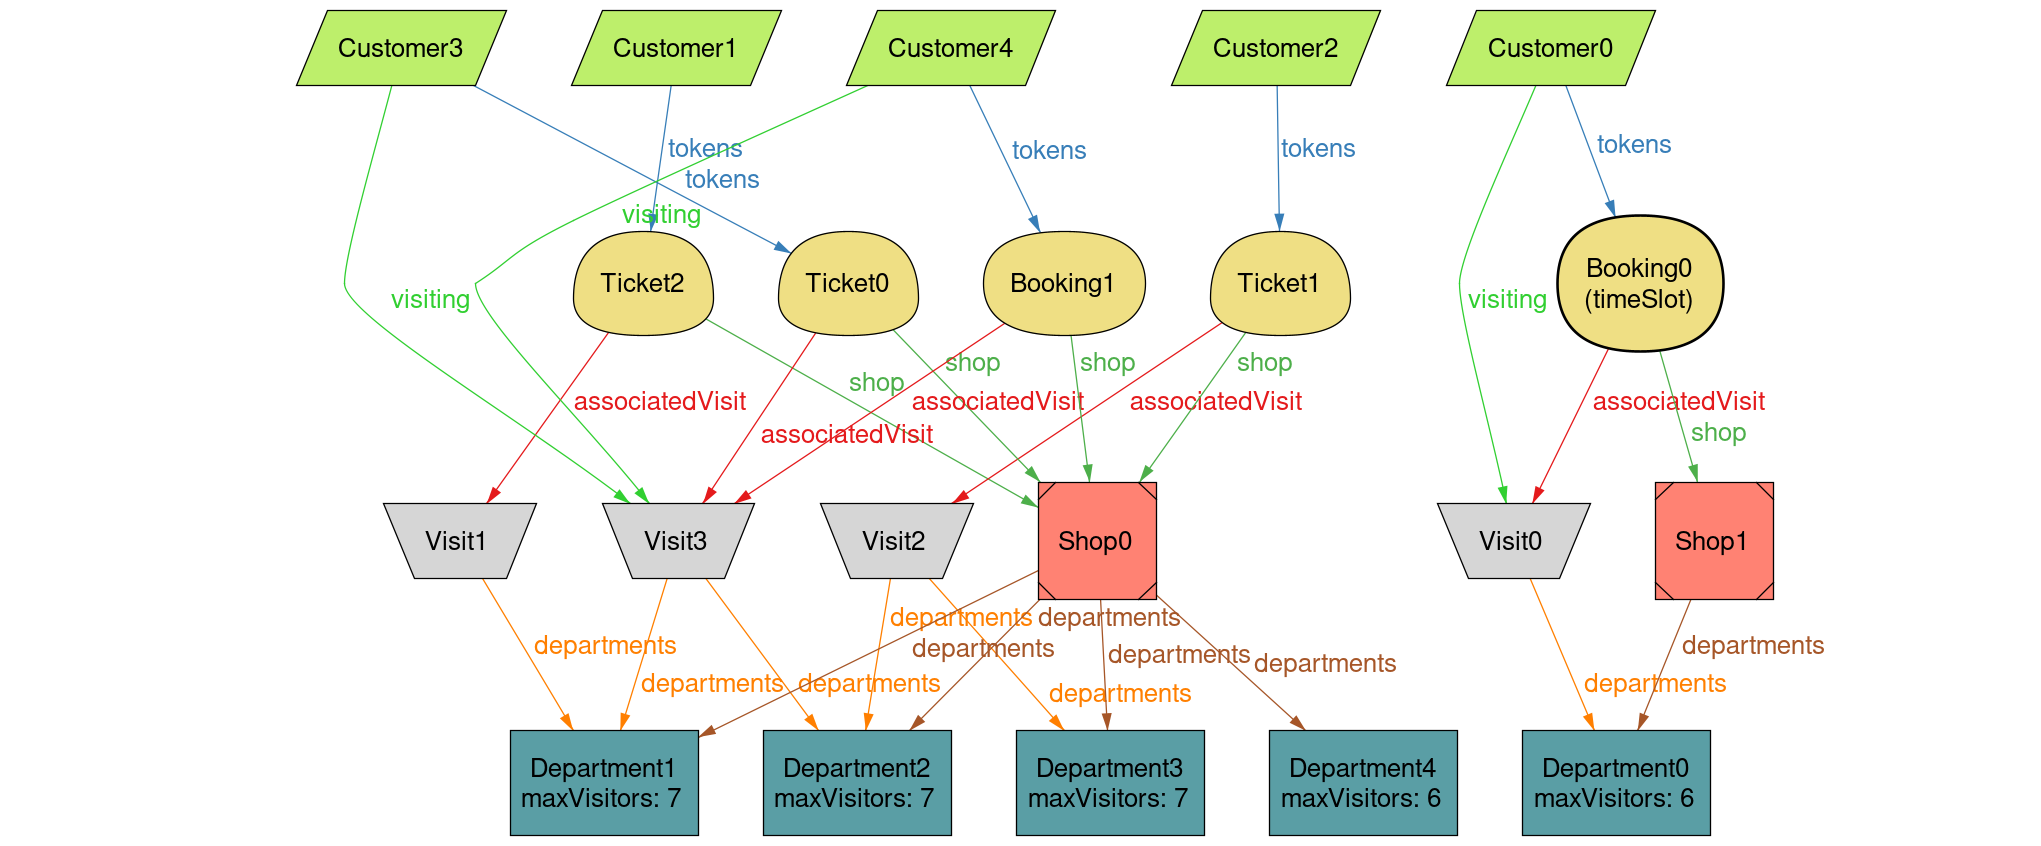
\includegraphics[height=0.25\textheight]{Images/Alloy/5Customers_v1_t3.png}
    \caption{Run for Time 3. \emph{Customer1} correctly exits \emph{Shop0}, while \emph{Customer0} makes use of a Booking for \emph{Shop1}}
\end{figure}
\begin{figure}[H]
    \centering
    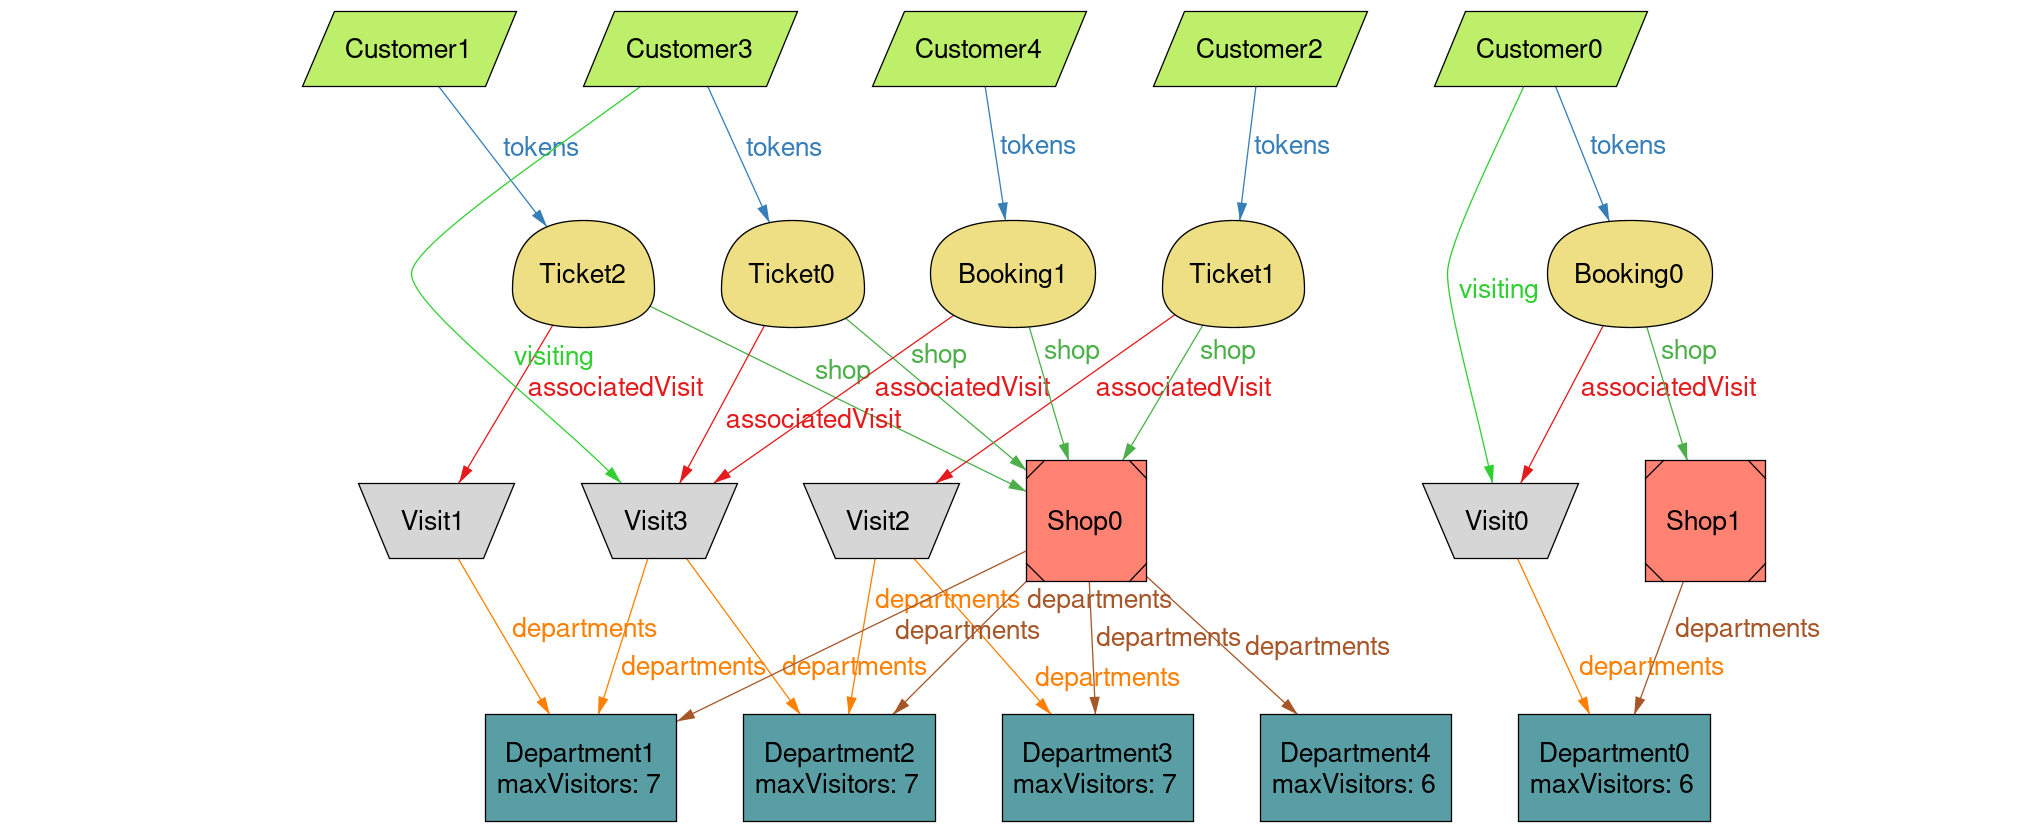
\includegraphics[height=0.25\textheight]{Images/Alloy/5Customers_v1_t4.png}
    \caption{Run for Time 4. \emph{Customer4} exits as well.}
\end{figure}

\pagebreak
Figure \ref{fig:waitinglistnode1} and \ref{fig:waitinglistnode2} provide a more detailed view of the same instance, displaying the working principle of the waiting List. Each WaitingListNode represents a single Customer in line, with their Ticket. In the first figure, set at Time 0, we see that \emph{Customer1} has the Ticket corresponding to the first WaitingListNode for \emph{Shop0}, pointed by the \emph{queue} attribute, thus he is allowed to enter at the next time frame.
Indeed, in the second figure, set at Time 1, a new \emph{visiting} connection between \emph{Customer1} and \emph{Visit1} is spawned, which means that the Customer is visiting \emph{Department1} of \emph{Shop0}. The \emph{queue} attribute of the Shop has also been moved forward to a new WaitingListNode, as expected.
\begin{figure}[H]
    \centering
    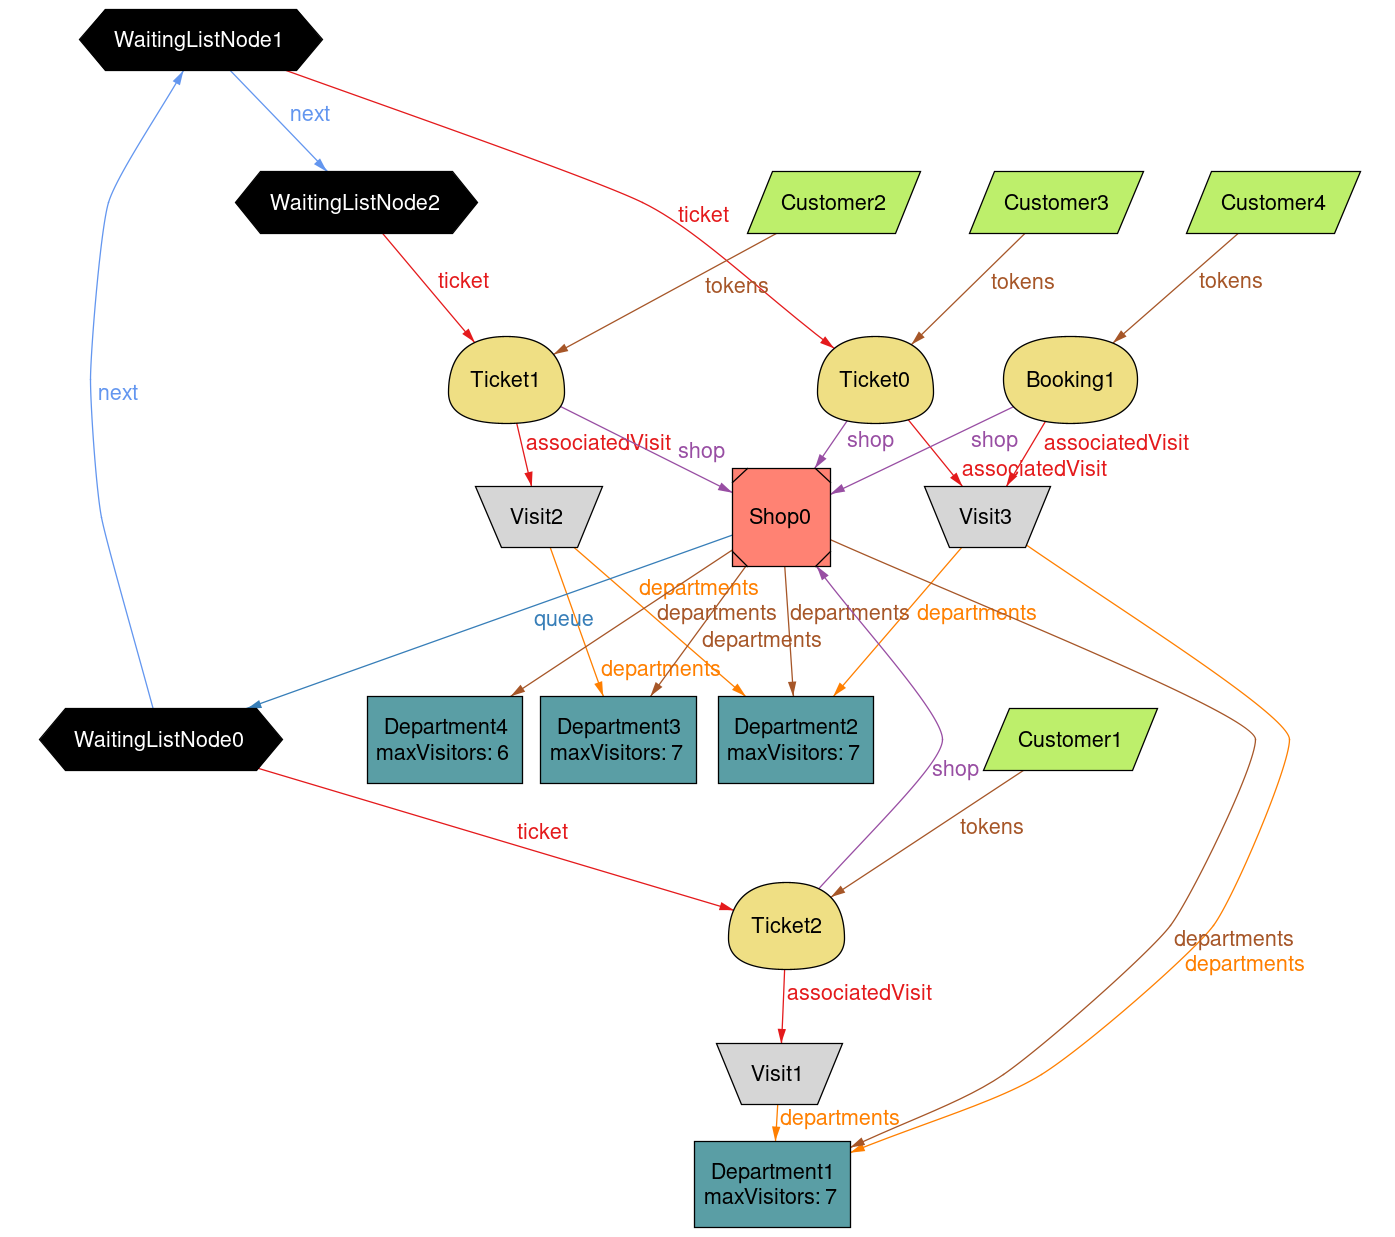
\includegraphics[width=\textwidth]{Images/Alloy/5Customers_v1_t0_detail_crop.png}
    \caption{The same instance at Time 0, with WaitingListNode elements shown}
    \label{fig:waitinglistnode1}
\end{figure}
\begin{figure}[H]
    \centering
    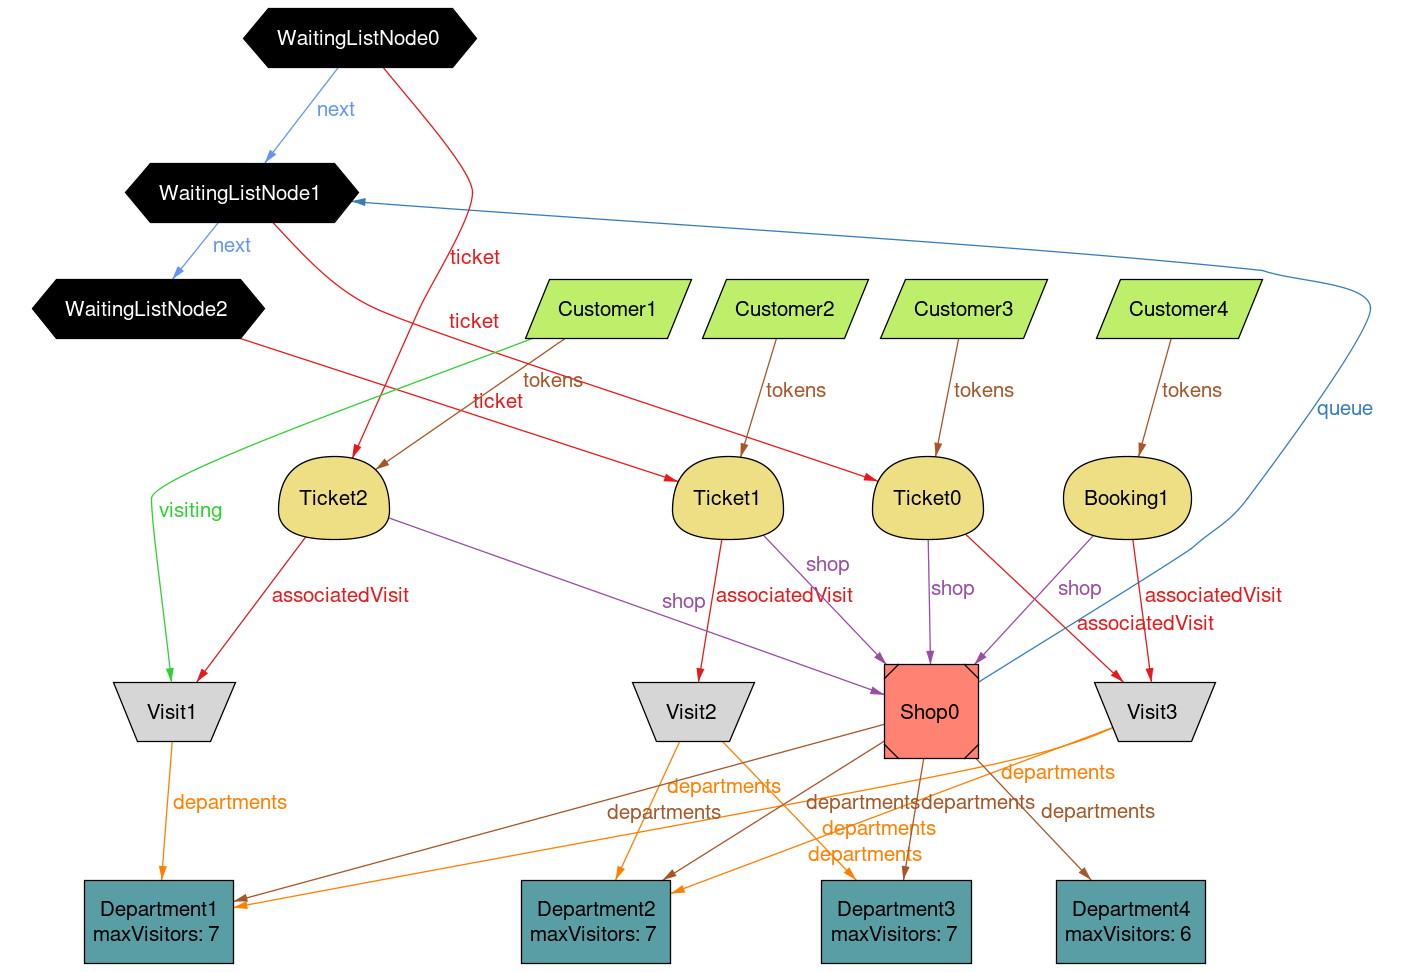
\includegraphics[width=\textwidth]{Images/Alloy/5Customers_v1_t1_detail_crop.png}
    \caption{The evolution of the instance at Time 1}
    \label{fig:waitinglistnode2}
\end{figure}